\section{Probabilistic catalogs based on the 3FGL and 4FGL catalogs}
\lb{sec:prob_cats}

In this section we use the ML algorithms optimized in the previous section to construct probabilistic
classification of sources in the 3FGL and 4FGL catalogs.
%Having optimized our algorithms, we decided to test them on 3FGL data which was initially unassociated but then became associated in 4FGL. Furthermore, we tested the algorithms on 4FGL associated data, and also predicted for unassociated data.


\subsection{Probabilistic classification of sources in 3FGL and comparison with 4FGL}
\lb{sec:3FGLprediction1}


%In this section we perform probabilistic classification of sources in the 3FGL catalog.
We use the following four algorithms for the classification of sources: RF with 50 trees and maximal depth of 6, BDT with 100 trees and maximal depth of 2, NN with 10 neurons, Adam solver, and 300 epochs, and LR with LBFGS solver and 200 iterations. 
For training we use the pulsars and AGNs from the 3FGL catalog. In addition to original datasets, we perform oversampling of pulsars in order to balance the numbers of pulsars and AGNs.
As a result, we have 8 classification methods: 4 algorithms train with or without oversampling.

The selected algorithms are summarized in Table \ref{tab:selected_algs}, where oversampling is shown by ``\_O''.
``Average testing accuracy'' is computed by taking 1000 times 70\% - 30\% split into training and testing samples and averaging over the 
accuracies computed for the testing samples.
In addition, we look at sources, which are unassociated in 3FGL but have either pulsar or AGN association in 4FGL: there are 278 such sources.
The accuracy of our prediction for the four selected algorithms with and without oversampling, taking the 4FGL classes as the true values, is reported in the column ``Comparison with 4FGL Accuracy''.
The correct classifications and misclassifications for the 278 sources with associations in 4FGL are also presented in Figure \ref{fig:3FGL_vs_4FGL_classes}.
The class at the beginning of the label names corresponds to the association in the 4FGL, while the second half of the labels corresponds to classification of unassociated sources in 3FGL. For example, ``PSRs classified only as PSRs'' shows sources which have PSR association in 4FGL and all four algorithms classified the corresponding unassociated sources in 3FGL as PSRs for both unweighted and oversampled training data. On the other hand ``PSRs classified as either PSRs or AGNs'' labels sources with PSR associations in 4FGL but the corresponding unassociated sources in 3FGL have both PSR and AGN classifications by different ML algorithms, again for both types of training data.
The unassociated sources are classified as PSRs or AGNs if the corresponding probability is larger than 0.5.
We notice that misclassified or partially misclassified sources in Figure \ref{fig:3FGL_vs_4FGL_classes} typically happen on the boundary between the two classes or even inside the opposite class.
Many of these sources also have flags in the 3FGL catalog, such as a potential problem with the background diffuse emission model in the location of the source, which can lead to a poor reconstruction of the source spectrum and, as a result, misclassification of the source.

%Here we discuss the results of our probabilistic classification on the unassociated data. The 242 sources for whom FGL counterparts existed were plotted in figure 10. This figure shows all AGNs and PSRs, including those which were correctly or incorrectly identified by all the 4 algorithms (given by keyword only) and those which are a mix of correct and incorrect classification by at least one of the 4 algorithms (given by keywords either/or). 



\begin{table}[!h]
\hspace{-0.2cm}
\resizebox{0.47\textwidth}{!}{
    \tiny
  \centering
    \renewcommand{\tabcolsep}{0.4mm}
\renewcommand{\arraystretch}{1.6}

%\hspace{-3mm}
    \begin{tabular}{|c|c|c|c|c|c|c|}
    \hline
    Algorithm&Parameters &  Testing&Std. Dev.& Comparison with 4FGL \\
    & & Accuracy & & Accuracy \\
    \hline
    RF & 50 trees, max depth 6  &97.42&0.60& 96.1  \\
    RF\_O &   &97.71&0.56& 95.1  \\
    \hline %\midrule   -> aakash do you mean this?
    BDT & 100 trees, max depth 2    &   97.80&0.55&95.34 \\
%    \hline %\midrule   -> aakash do you mean this?
%    BDT & 200 trees, max depth 2    &   95.8  \\
    BDT\_O &     &   97.82&0.51& 93.8 \\
    \hline
    NN & 300 epochs, 10 neurons, Adam & 97.40&0.87& 94.55\\
    NN\_O &  & 95.96&0.84& 91.43\\
    \hline
    LR & 200 iterations, LBFGS solver & 97.60&0.56& 93.48 \\
    LR\_O &  & 94.01&0.97& 87.07 \\
    \hline
     
    \end{tabular}}
    \vspace{2mm}
    \caption{Accuracy of the 4 selected algorithms for classification of 3FGL sources.}
    \label{tab:selected_algs}
\end{table}

\begin{figure*}[h]
\centering
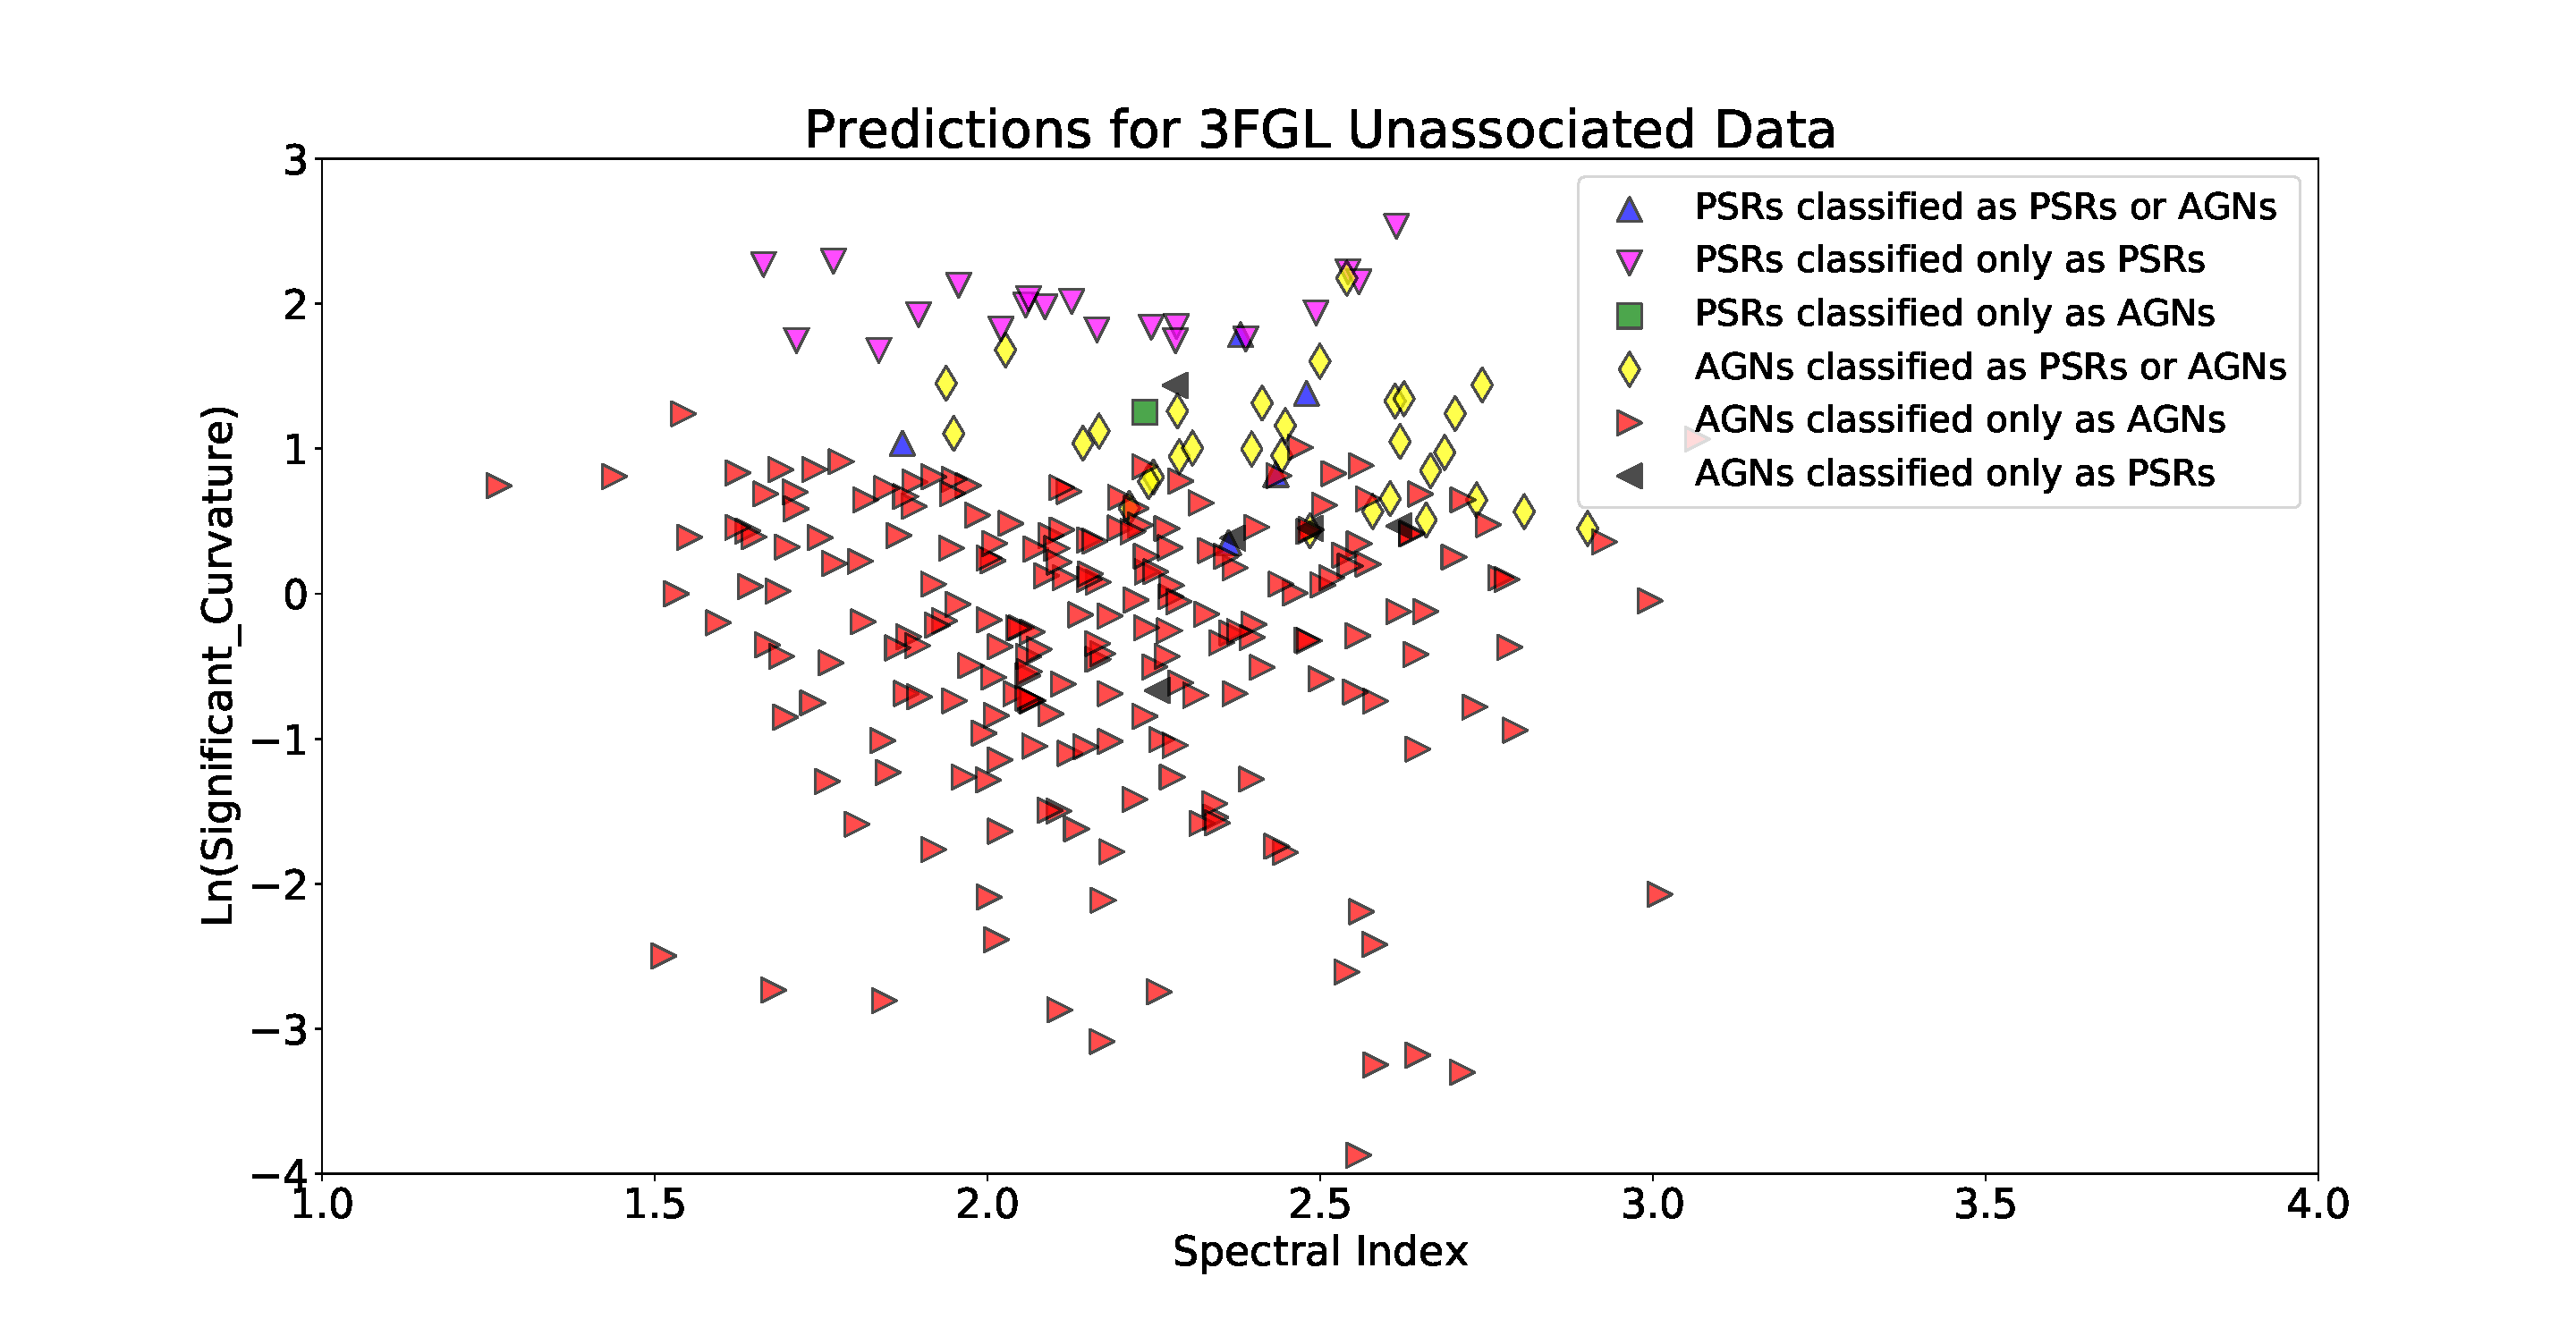
\includegraphics[width=0.8\textwidth]{plots/finalclassification_3fglvs4fgl.pdf}
%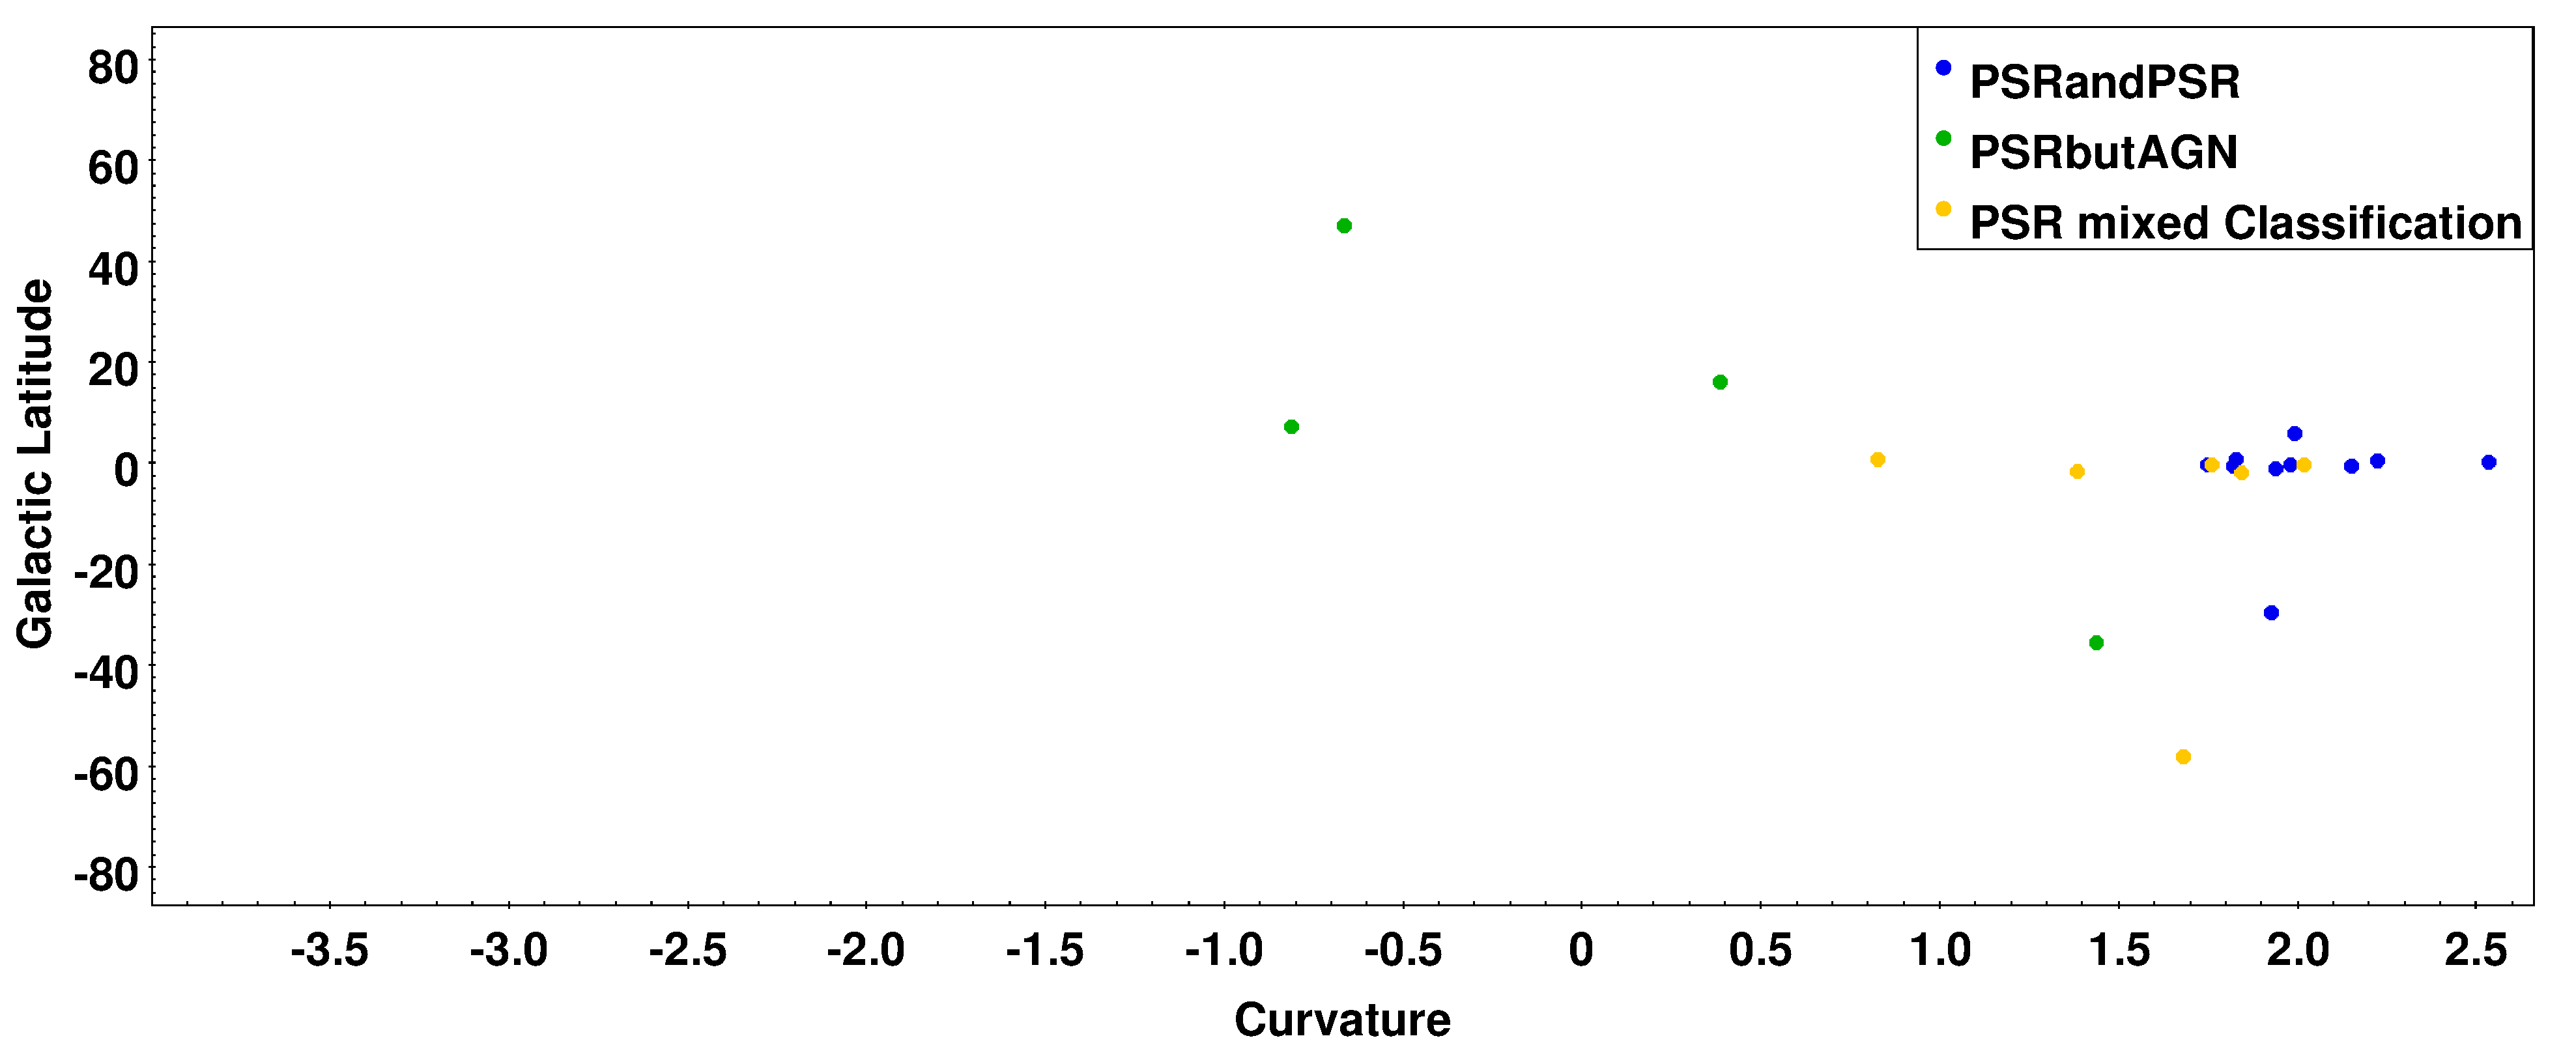
\includegraphics[width=\twopicsp\textwidth]{plots/PSR3.pdf}
\caption{Comparison of class prediction for unassociated 3FGL sources with classes in 4FGL. }
%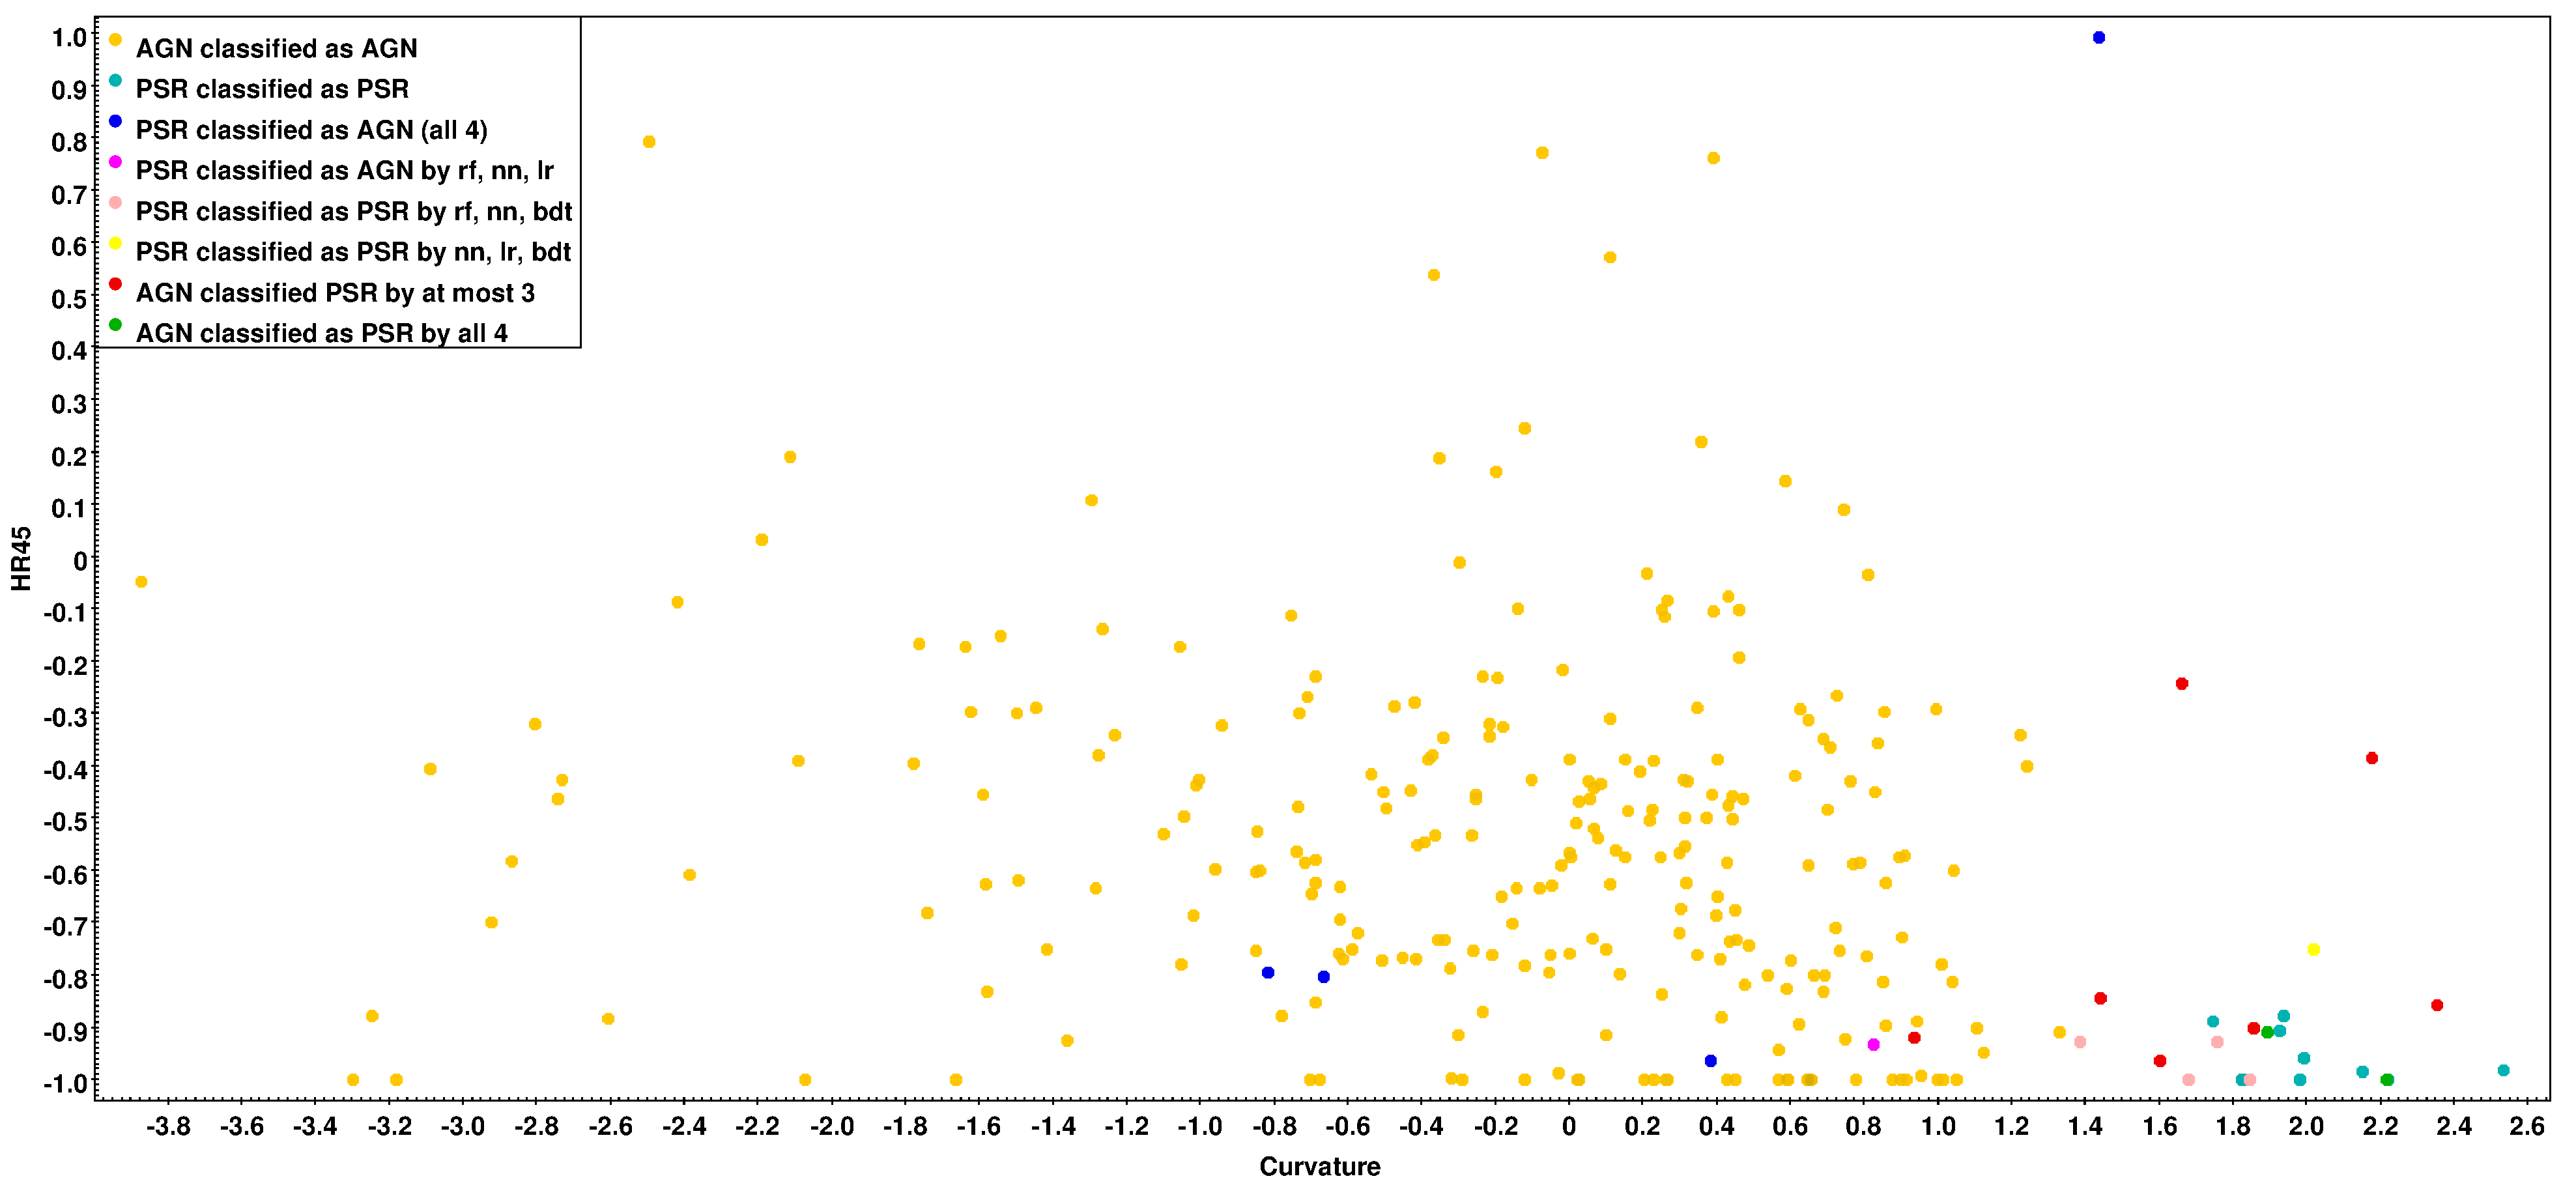
\includegraphics[width=\twopicsp\textwidth]{plots/final_catalog.pdf}
\label{fig:3FGL_vs_4FGL_classes}
\end{figure*}

As a result of the classification with the four ML algorithms,
we created a probabilistic catalog based on the 3FGL sources without missing values.%
\footnote{There are thirteen sources with missing values in the 3FGL catalog, which we save in a separate file ``3FGL\_sources\_with\_missing\_values.csv'' for reference.}
We train on 70\% of the sources associated with pulsars or AGNs and save the probability values for training sources, sources which are not classified as pulsars or AGNs, and for unassociated sources.
We repeat the splitting and training 1000 times and report the sample average and standard deviation of the classification probabilities,
i.e., we average over 1000 values for unassociated sources and sources not classified as AGNs or pulsars, 
while the average for AGNs and pulsar is over the number of times the sources appear in the training sample, which is about 300.
%Like in the case of associated sources, where we split the data 1000 times, we also do a 1000 runs for the unassociated case. This allows us to calculate individual probabilities and their standard deviations for all sources.
%\dima{Classification of associated sources is done by averaging over testing-training samples splits.
%Do we also do averaging for unassociated sources?}

We have also subselected the 278 unassociated 3FGL sources, which have PSR or AGN associations in 4FGL,
and saved them for convenience of comparison as a separate file.
In the probabilistic catalogs we add columns with corresponding probabilities for each algorithm and each class,
i.e., provided that there are 8 methods (including oversampling) and 2 classes, we add 16 columns: 8 for unweighted and 8 for oversampled training data respectively. The columns with '\_O' represent the oversampled probabilities. We also add 16 columns for standard deviations of probabilities. Although class probabilities and standard deviation for each algorithm are not independent (probabilities add up to 1 and standard deviations are equal for AGNs and PSRs), we keep the corresponding columns in view of possible generalizations to multi-class classification.
%Although the class probabilities for each algorithms should add up to one for every source, we still keep the columns for all classes for convenience.
Table \ref{tab:prob_cat} shows an example of the probabilistic catalog for a few unassociated 3FGL sources.
Notice that the first source is classified as a pulsar by BDT and as an AGN by RF, LR, and NN algorithms,
it is an example of a source with mixed classification.
%i.e., it has a label ``classified either as PSRs or AGNs'' in Figure \ref{fig:3FGL_vs_4FGL_classes}. - is it associated in 4FGL?
%The second and third sources are classified as AGNs by all four algorithms, i.e., they will have a label ``classified only as AGNs'',
%while the last source is classified as a pulsar by all four algorithms, i.e., it will have a label ``classified only as PSRs''.
Out of 1008 unassociated sources in 3FGL, 96 are classified as pulsars by all eight methods, 580 are classified as AGNs, and 332 have mixed classifications.
Out of 96 sources classified as pulsars, 6 sources have counterparts in Parkes survey \cite{Camilo2015} within 2 arc minutes (see Table \ref{tab:parkes}).

We summarize the results of classification of the unassociated 3FGL sources in Table \ref{tab:3FGL_prediction}.
The ``AGNs'' column shows the number of unassociated sources where all eight methods from table \ref{tab:selected_algs2} give the probability for a source to be an AGN above 50\%.
Similarly the ``Pulsars'' column shows the number of unassociated sources where all four algorithms predict the source to be more likely a pulsar.
The ``Mixed'' column shows the number of sources with mixed classification, i.e., some algorithms predict that the source is more likely an AGN while the other algorithms predict that it is more likely a pulsar.
In the ``Uncorrected'' row we do not take into account that there can be sources other than AGNs or pulsars among the unassociated sources.
We correct for the presence of the other sources by assuming that the fraction of AGN-like and pulsar-like sources among the other sources is the same for associated and for unassociated sources.
In particular, we denote by $N_{\rm AGN}$ the number of unassociated sources with AGN-like classification by all four algorithms,
by $N_{\rm AGN}^{\rm ass\,other}$ the number of sources with AGN-like classification among associated other sources,
by $N_{\rm ass}$ ($N_{\rm unass}$) the total number of associated (unassociated) sources.
The number of AGN-like sources among the unassociated source corrected for the presence of other sources is estimated as

\be
\lb{eq:other_correction}
N_{\rm AGN}^{\rm corr} = N_{\rm AGN} - N_{\rm AGN}^{\rm ass\,other} \,\frac{N_{\rm unass}}{N_{\rm ass}}.
\ee
Analogous corrections are applied for the number of unassociated sources with pulsar-like classification by all eight methods,
and for unassociated sources with mixed classification.




\pgfplotstableread[col sep=comma]{tables/3FGL_unassoc_vs_4FGL_assoc.csv}\loadedtable
\begin{table}
\pgfplotstabletypeset[columns={Source_Name_3FGL,AGN_BDT,AGN_RF,AGN_LR,AGN_NN},
column type=l,
string type,
every head row/.style={before row={\toprule & \multicolumn{4}{c}{AGN Probability} \\},after row=\midrule,},
every last row/.style={after row=\midrule}, %\vdots },
columns/Source_Name_3FGL/.style={column name=Source\_Name},
columns/AGN_BDT/.style={column name=BDT,numeric type,fixed,precision=3},
columns/AGN_NN/.style={column name=NN,numeric type,fixed,precision=3},
columns/AGN_RF/.style={column name=RF,numeric type,fixed,precision=3},
columns/AGN_LR/.style={column name=LR,numeric type,fixed,precision=3},
skip rows between index={4}{242}
]\loadedtable
\caption{\label{tab:prob_cat}
Example of the AGN classification probabilities for a few unassociated sources in the 3FGL catalog.}
\end{table}




\pgfplotstableread[col sep=comma]{tables/3fgl_unassoc_predictions_matches_with_Parkes(2015)_1.csv}\loadedtable
\begin{table}
\pgfplotstabletypeset[columns={3FGL,GLON,GLAT,Separation},
every head row/.style={before row={\toprule},after row=\midrule,},
every last row/.style={after row=\midrule },
columns/3FGL/.style={column name=Source\_Name,string type},
columns/GLON/.style={column name=GLON,numeric type,fixed,precision=1},
columns/GLAT/.style={column name=GLAT,numeric type,fixed,precision=1},
columns/Separation/.style={column name=Sep (arksec),numeric type,fixed,precision=1}
]\loadedtable
\caption{\label{tab:parkes}
Connection of unassociated 3FGL sources classified as PSRs with Parkes PSRs.}
\end{table}



\begin{table}[!h]
\resizebox{0.45\textwidth}{!}{
    \tiny
 %  \centering
    \renewcommand{\tabcolsep}{0.3mm}
\renewcommand{\arraystretch}{1.5}

    \begin{tabular}{| l |c|c|c|}
    \hline
    Correction for other sources & AGNs & Pulsars & Mixed \\
    \hline
    Uncorrected &  580 & 96  &  332 \\
    \hline
    Corrected & 561.5  & 83.0  & 309.5 \\
    \hline
     
    \end{tabular}}
    \vspace{0.2cm}
    \caption{Expected number of AGNs and pulsars among the unassociated 3FGL sources.
    ``AGNs'' and ``Pulsars'' columns show the number of sources where all four algorithms predict the same class,
    ``Mixed'' column shows the number of sources with mixed classification.
    Uncorrected (corrected) rows show the number of predicted AGNs and pulsars among the unassociated sources, which are
    uncorrected (corrected) for the presence of sources other than AGNs and pulsars among the unassociated sources.}
    \label{tab:3FGL_prediction}
\end{table}



\subsection{Probabilistic classification of sources in the 4FGL catalog}
\lb{sec:4FGLprediction}

In this section we construct a probabilistic classification of sources in the 4FGL catalog \citep{2020ApJS..247...33A}.%
\footnote{There is also a version of the 4FGL catalog based on 10 years of data, rather than 8 years of data: the 4FGL-DR2 catalog
\citep{2020arXiv200511208B}. We discuss our predictions for 4FGL-DR2 in Section \ref{sec:4FGL-DR2}.}
As in the previous section, we use for training and testing sources associated with either AGNs or pulsars,
which have no missing values used for classification.%
\footnote{Overall, in the 4FGL catalog there is only one source with missing values: 4FGL J0534.5+2201i associated with the Crab pulsar wind nebula.}
We then calculate the classification probabilities of AGN and PSR classes for both the associated and the unassociated sources.
The 4FGL catalog has higher number of features, especially due to the difference in modeling of the spectra compared with the 3FGL catalog. 
We selected 31 of these features and looked for correlations among them. If any feature was correlated or anti-correlated with a Pearson index of $\pm$0.75 or higher with another feature, then only one of these features was kept. 
%The correlation matrix is shown in Figure \ref{fig:corr_mat}.
The resulting 16 features are:
GLON, GLAT, ln(Pivot\_Energy), ln(Flux1000), PL\_Index, Unc\_LP\_Index, LP\_beta, LP\_SigCurv, Unc\_PLEC\_Expfactor, PLEC\_Exp\_Index, hr12, hr23, hr34, hr45, hr56, hr67, ln(Variability\_Index).
Some of these features are directly related to the features, which we use in the 3FGL catalog,
e.g., GLAT, PL\_Index (instead of Spectral\_Index), LP\_SigCurv (instead of ln(Signif\_Curve)), 
ln(Variability\_Index), hardness ratios (in the 4FGL catalog there are two more energy bins compared to the 3FGL catalog).

\begin{comment}
\begin{figure*}[h]
\centering
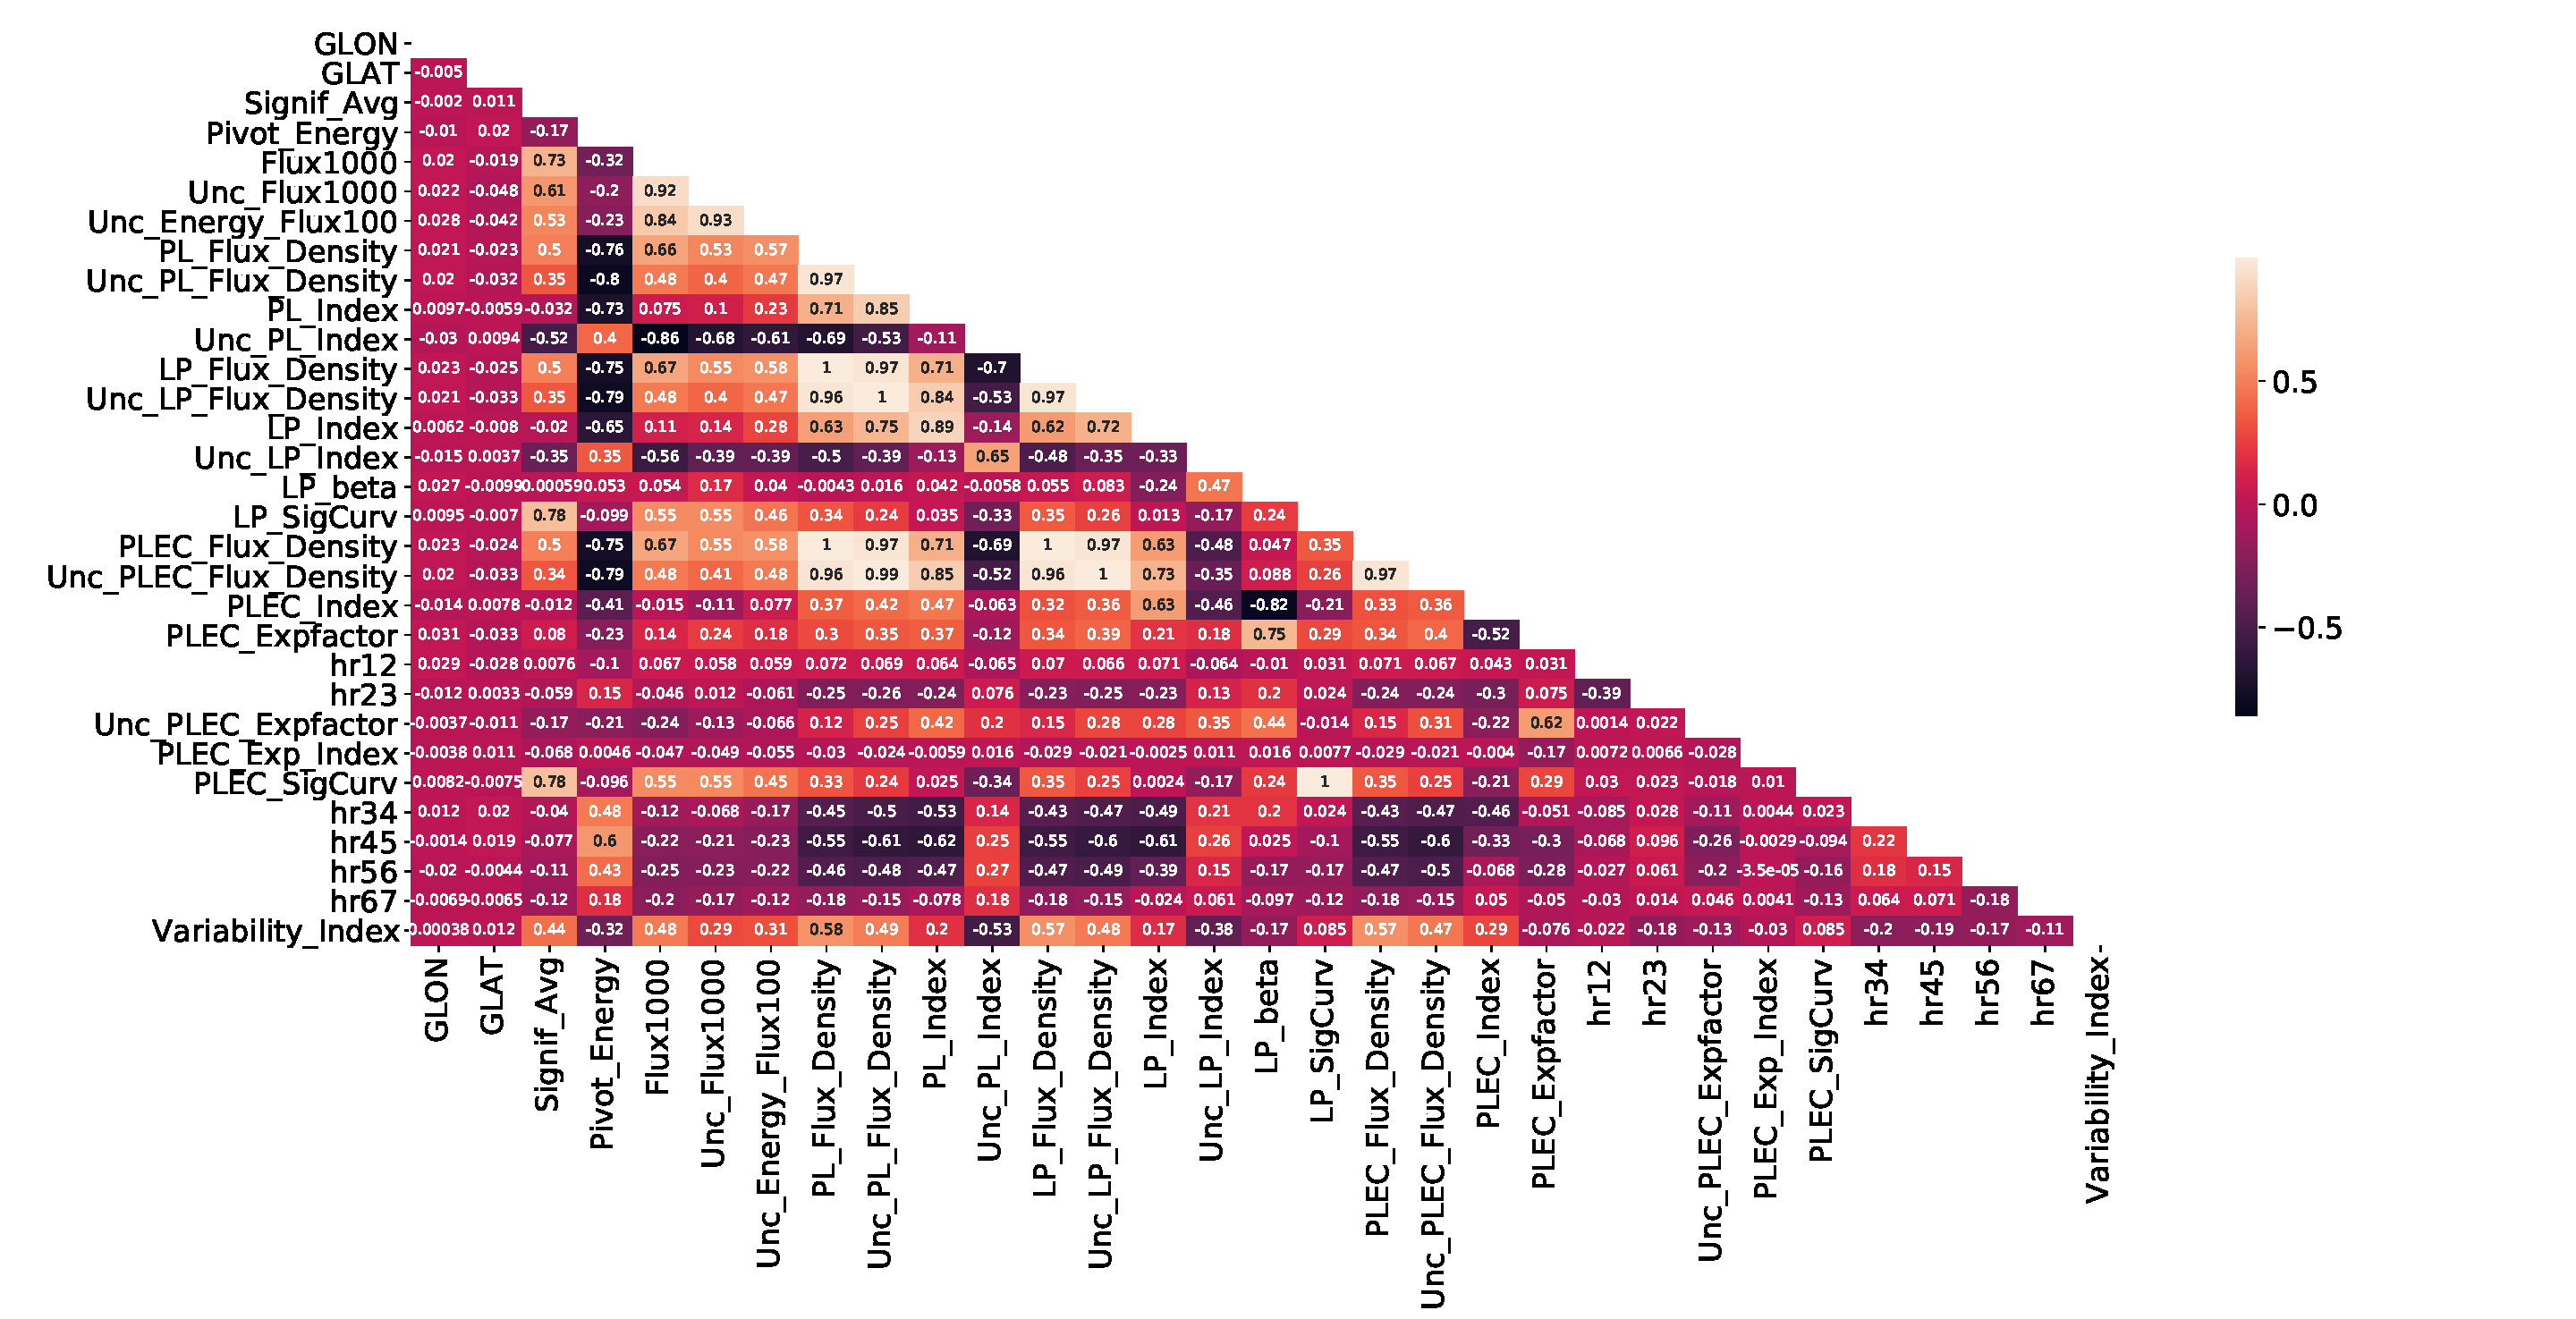
\includegraphics[width=\textwidth]{plots/correlation_4fgl_assoc.pdf}
%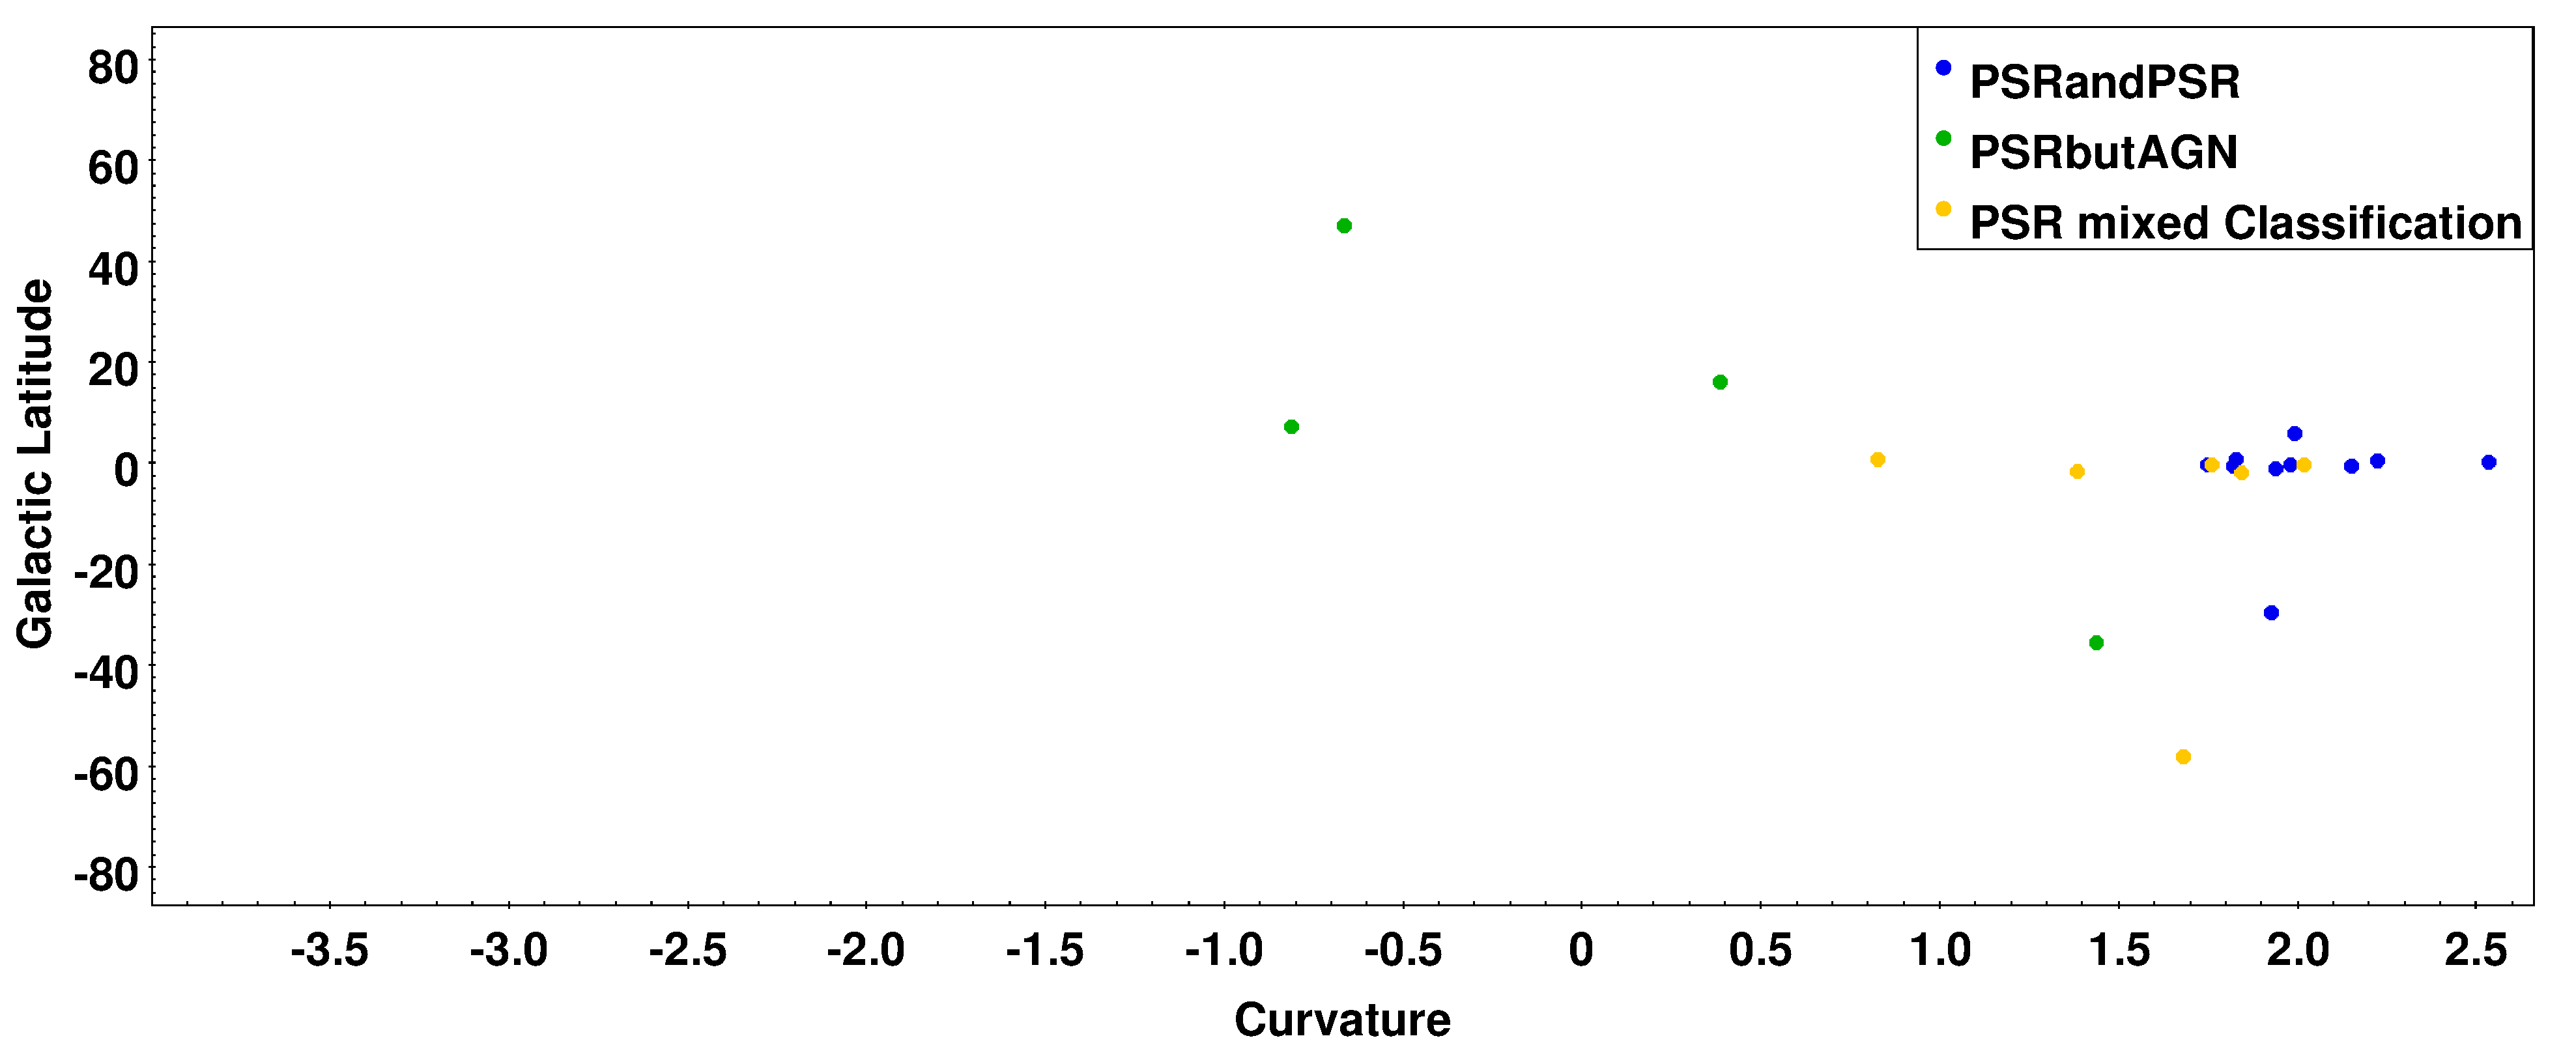
\includegraphics[width=\twopicsp\textwidth]{plots/PSR3.pdf}
\caption{Corelation matrix for 4FGL associated data }
%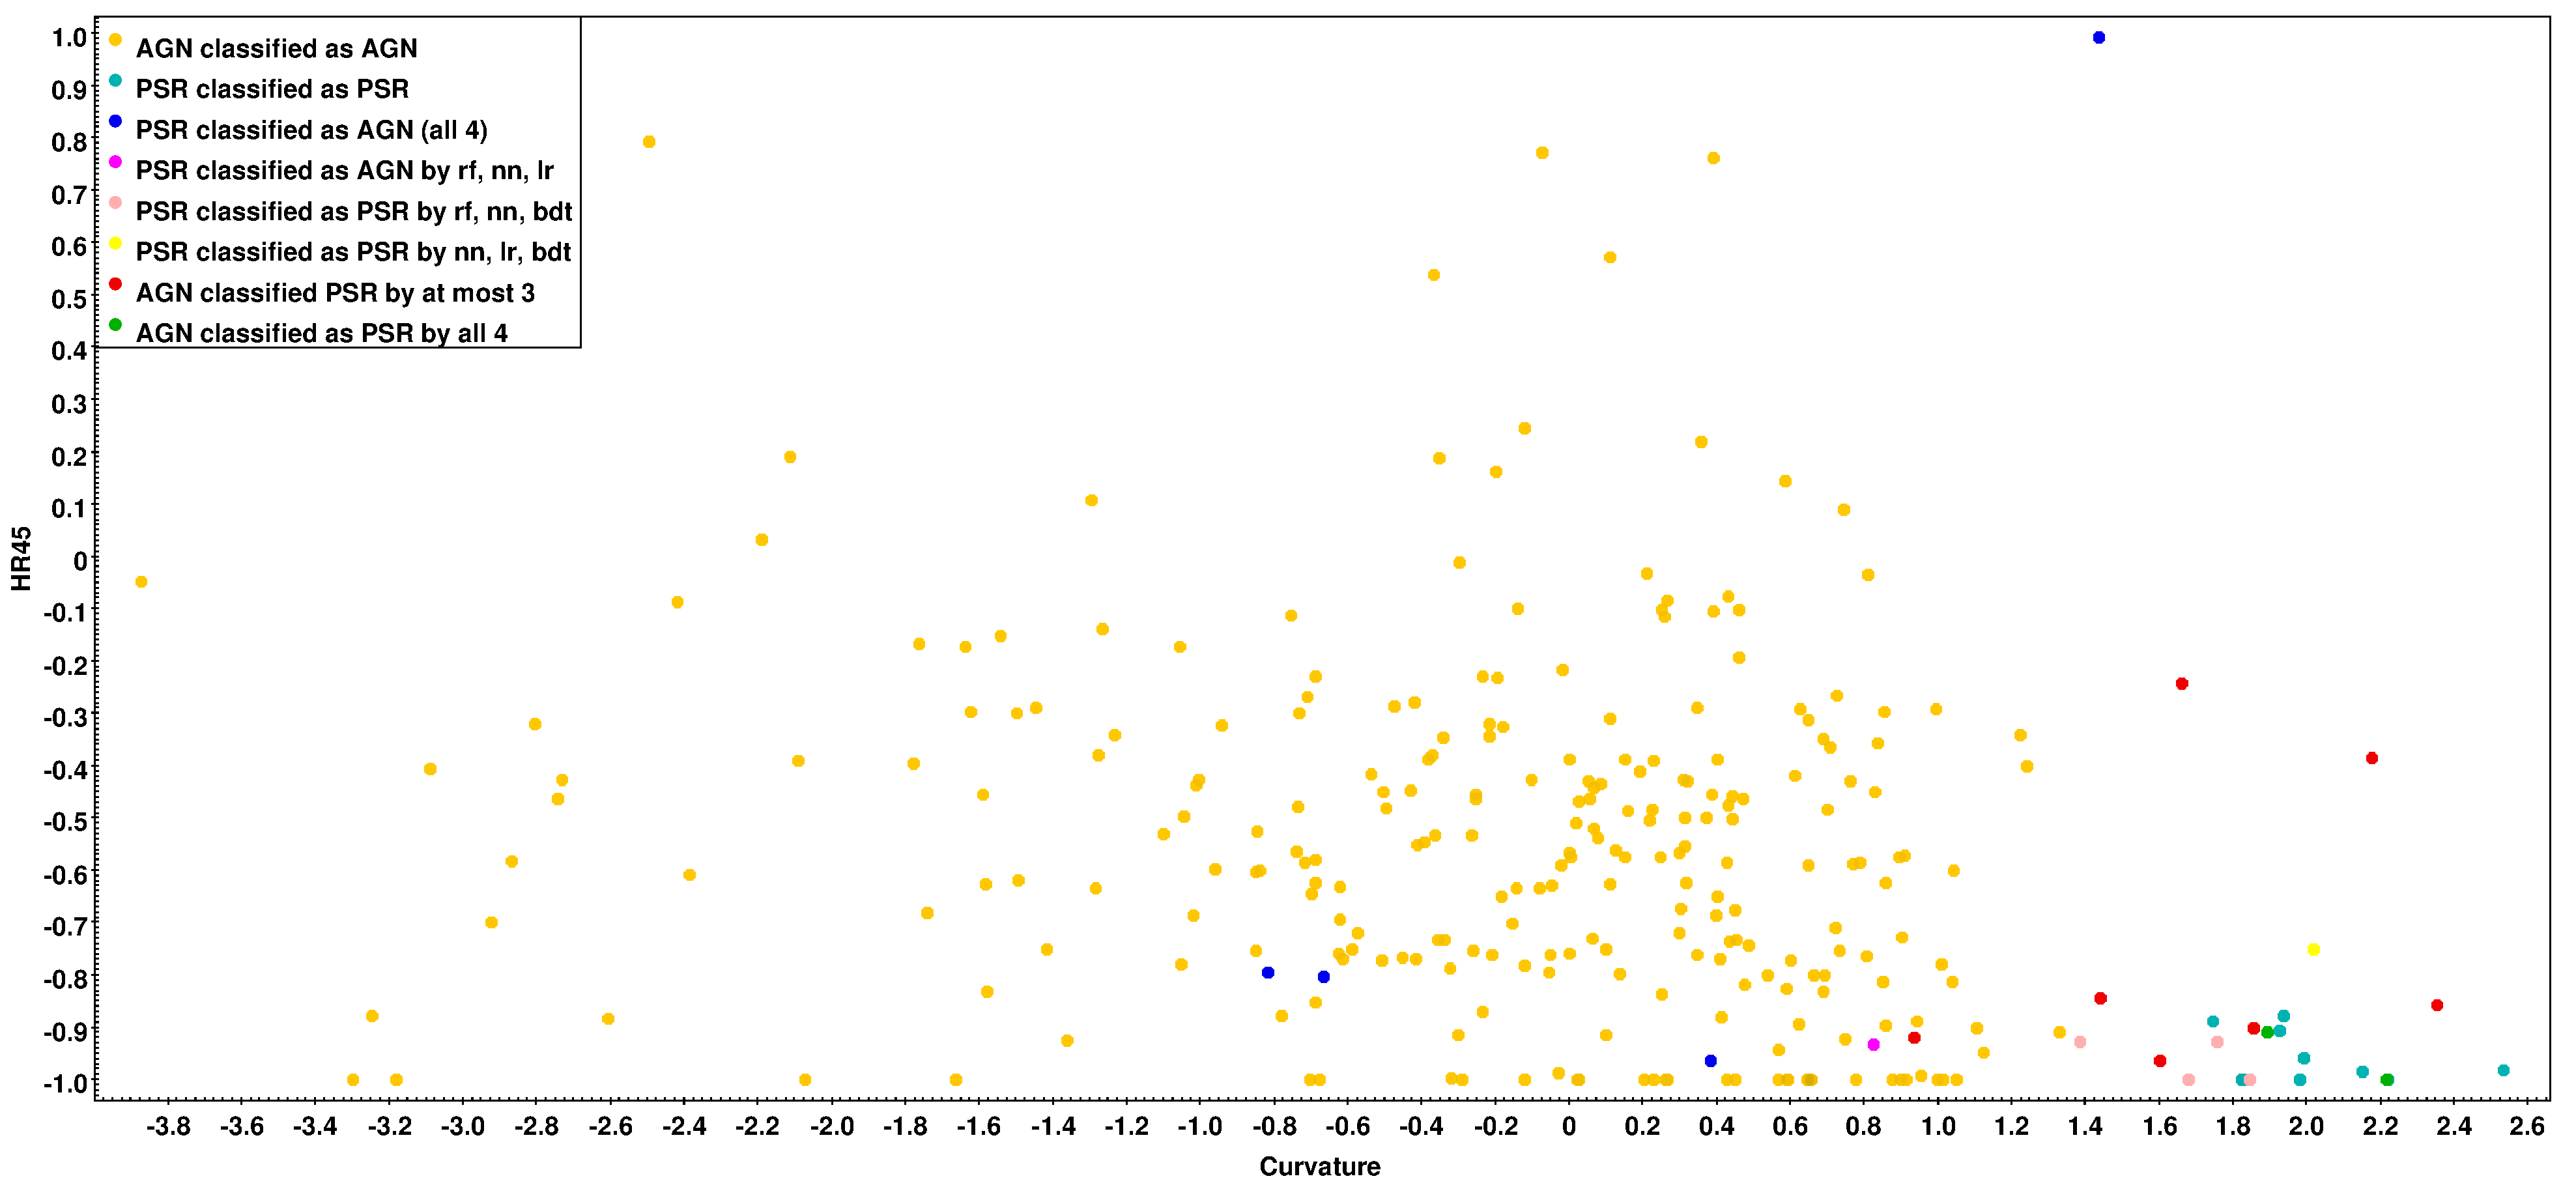
\includegraphics[width=\twopicsp\textwidth]{plots/final_catalog.pdf}
\label{fig:corr_mat}
\end{figure*}
\end{comment}

For this part, we do not perform another preliminary analysis of the algorithms, i.e., we used the same hyper-sparameters for the four algorithms as in the construction of the probabilistic catalog based on the 3FGL catalog, except for NN where we increased the number of neurons in the first hidden layer to 16. Similarly to the construction of the 3FGL probabilistic catalog, we use both unweighted training samples and oversampling, i.e., we have 8 classification algorithms.
We retrain these algorithms using the 16 features for the 4FGL sources.
The corresponding accuracies are reported in Table \ref{tab:selected_algs2}.
All algorithms have a slightly better accuracy for the 4FGL catalog compared to the 3FGL catalog, which is likely due to a higher number of features and more associated sources used as training data. 

% (same as the number of features). However, due to the number of features being higher, we hypothesized that the Neural Network should under-perform as compared to before.

\begin{table}[!h]
\resizebox{0.45\textwidth}{!}{
    \tiny
 %  \centering
    \renewcommand{\tabcolsep}{0.4mm}
\renewcommand{\arraystretch}{1.6}

    \begin{tabular}{|c|c|c|c|}
    \hline
    Algorithm&Parameters & Testing Accuracy & Std. Dev.\\
    \hline
    RF& 50 trees, max depth 6  &98.27 & 0.35\\
    RF\_O   &&98.12&0.37 \\
    \hline
    NN & 300, 16 Neurons, Adam & 98.08 & 0.39\\
    NN\_O&&97.17&0.55\\
    \hline %\midrule   -> aakash do you mean this?
    BDT & 100 trees, max depth 2    &   98.23 &0.40\\
    BDT\_O&&98.15&0.36\\
%    \hline %\midrule   -> aakash do you mean this?
%    BDT & 200 trees, max depth 2    &   95.8  \\
    \hline
    LR & LBFGS solver, 200 iterations & 98.08&0.35\\
    LR\_O&&96.67&0.53\\
    \hline
     
    \end{tabular}}
    \vspace{0.2cm}
    \caption{Accuracy of the 4 selected algorithms on 4FGL associated data.}
    \label{tab:selected_algs2}
\end{table}

The expected numbers of AGNs and pulsars among the unassociated source in the 4FGL catalog are reported in Table \ref{tab:4FGL_prediction}.
The definition of columns and rows is the same as in the 3FGL catalog case in Section \ref{sec:3FGLprediction1}.

\begin{table}[!h]
\resizebox{0.45\textwidth}{!}{
    \tiny
 %  \centering
    \renewcommand{\tabcolsep}{0.3mm}
\renewcommand{\arraystretch}{1.5}

    \begin{tabular}{| l |c|c|c|}
    \hline
    Correction for other sources & AGNs & Pulsars & Mixed \\
    \hline
    Uncorrected &  674 & 141  &  521 \\
    \hline
    Corrected & 638.5  & 119.1  & 475.5 \\
    \hline
     
    \end{tabular}}
    \vspace{0.2cm}
    \caption{Expected numbers of pulsars and AGNs among unassociated sources in the 4FGL catalog.
    For definitions see Table \ref{tab:3FGL_prediction}.}
    \label{tab:4FGL_prediction}
\end{table}

Finally, we looked at sources which were unassociated in both 3FGL and 4FGL. Out of 306 such sources, 38 sources are predicted to be pulsars using 3FGL features and 71 sources are predicted to be pulsars using 4FGL features. This leads to 29 sources which were predicted by all eight methods to be pulsars for features taken from both 3FGL and 4FGL catalogs. Among these 29 sources, four can be spatially associated to pulsars in the Parkes survey (of the other two, one is now associated as a pulsar in 4FGL, and the second one is not detected in 4FGL).  For convenience, we save these 29 pulsar candidates as a separate file.



\subsection{Probabilistic classification of sources in the 4FGL-DR2 catalog}
\lb{sec:4FGL-DR2}

The 4FGL-DR2 catalog \citep{2020arXiv200511208B} 
is based on 10 years of \Fermi-LAT data \citep[compared to 8 years of data in the 4FGL catalog,][]{2020ApJS..247...33A}.
It contains 5788 sources, which is 723 more sources than in the 4FGL catalog (all sources in 4FGL are kept in 4FGL-DR2 even if they happen to be below the detection threshold with 10 years of data).
There are 14 sources in 4FGL-DR2 with missing values: four AGNs, one PWN (Crab), and nine unassociated sources.
The expected numbers of pulsars and AGNs among the 1670 unassociated sources in 4FGL-DR2 without missing values are
presented in Table \ref{tab:4FGL-DR2}.
Correction for the presence of other sources is calculated similarly to the 3FGL calculation in Section \ref{sec:3FGLprediction1}.
We find that compared to the 4FGL catalog, there are more sources classified as AGNs and sources with mixed classification among the unassociated source in 4FGL-DR2, whereas the numbers of sources classified as pulsars in 4FGL and 4FGL-DR2 are similar.

\begin{table}[!h]
\resizebox{0.45\textwidth}{!}{
    \tiny
 %  \centering
    \renewcommand{\tabcolsep}{0.3mm}
\renewcommand{\arraystretch}{1.5}

    \begin{tabular}{| l |c|c|c|}
    \hline
    Correction for other sources & AGNs & Pulsars & Mixed \\
    \hline
    Uncorrected &  854 & 144  &  672 \\
    \hline
    Corrected & 801.9  & 120.8  & 602.0 \\
    \hline
     
    \end{tabular}}
    \vspace{0.2cm}
    \caption{Expected numbers of pulsars and AGNs among unassociated sources in the 4FGL-DR2 catalog.
    For definitions see Table \ref{tab:3FGL_prediction}.}
    \label{tab:4FGL-DR2}
\end{table}
